\section{Decision Networks}
\textbf{MEU}: Choose the action which maximizes the expected utility given the evidence. \\
Decision networks are just Bayes' Nets with extra node types for actions and utilities. Action nodes cannot have parents and act as observed evidence, while utility nodes depend on action and chance nodes. \\
\textbf{Value of (Perfect) Information}: Value of acquiring evidence, can be done directly from decision network. VPI is nonnegative, nonadditive (meaning that typically, but not always, $\text{VPI}(E_j,E_k|e)\neq\text{VPI}(E_j|e)+\text{VPI}(E_k|e)$), and order-independent ($\text{VPI}(E_j,E_k|e)=\text{VPI}(E_j|e)+\text{VPI}(E_k|e,E_j)=\text{VPI}(E_k|e)+\text{VPI}(E_j|e,E_k)$).
\begin{figure}[H]
\centering
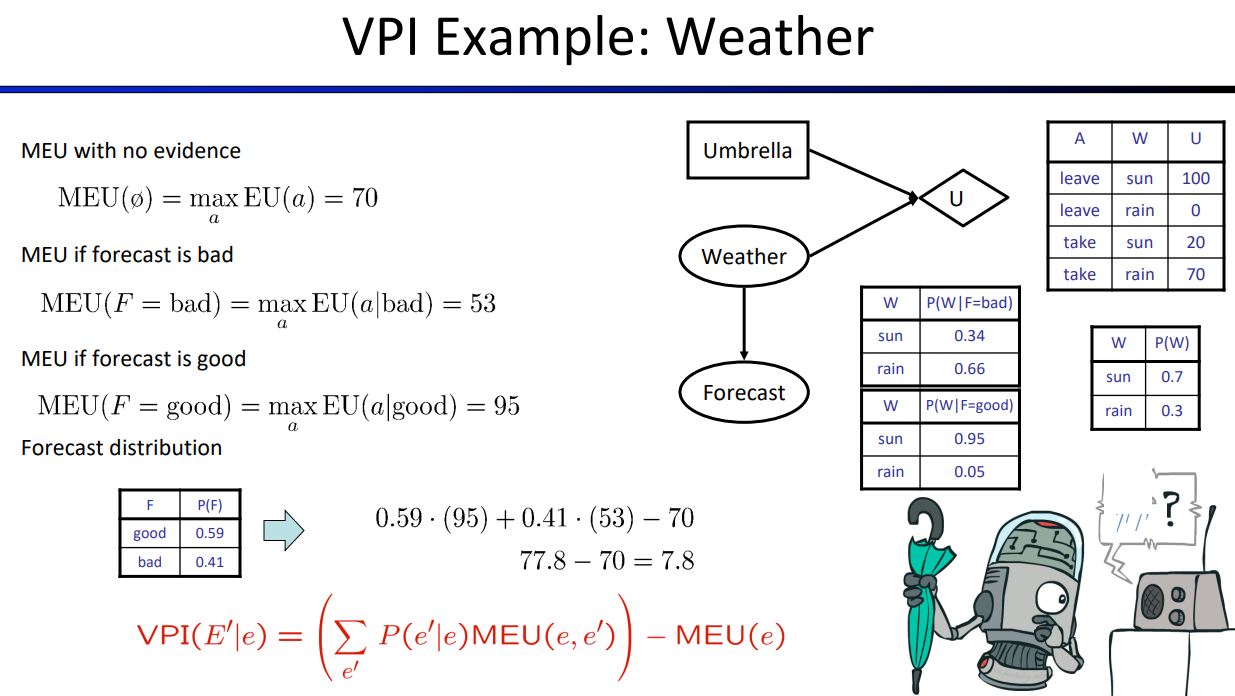
\includegraphics[width=\linewidth]{vpi-example-1}
\end{figure}
\begin{figure}[H]
\centering
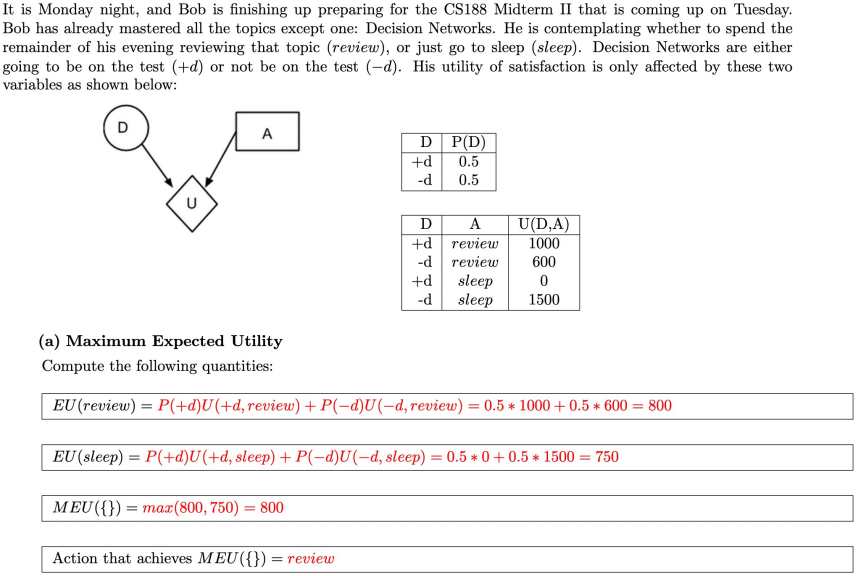
\includegraphics[width=\linewidth]{decision-network-exercises-1}
\end{figure}
\begin{figure}[H]
\centering
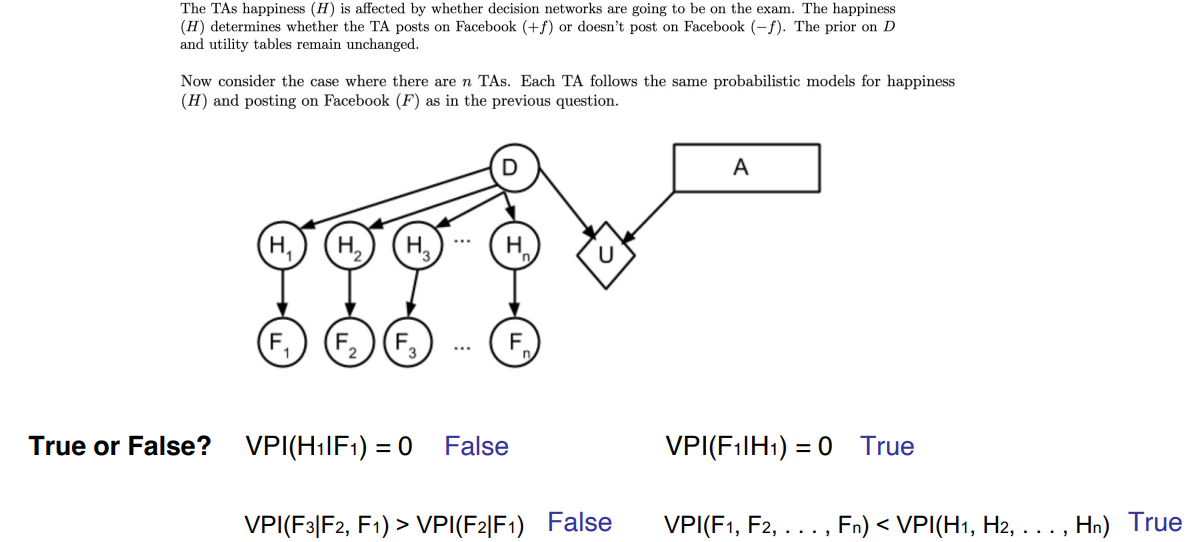
\includegraphics[width=\linewidth]{decision-network-exercises-2}
\end{figure}